\documentclass[tikz,border=3.14mm]{standalone}
\usetikzlibrary{positioning,chains}
\colorlet{myred}{red!80!black}
\colorlet{myblue}{blue!80!black}
\colorlet{mygreen}{green!60!black}
\colorlet{mydarkred}{myred!40!black}
\colorlet{mydarkblue}{myblue!40!black}
\colorlet{mydarkgreen}{mygreen!40!black}
\begin{document}
    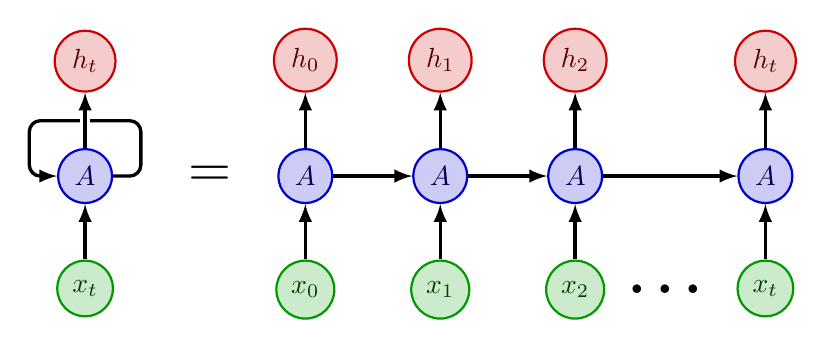
\begin{tikzpicture}[item/.style={circle,draw,thick,align=center}, itemc/.style={item,on chain,join}]
    \begin{scope}[start chain=going right,nodes=itemc,every
    join/.style={-latex,very thick},local bounding box=chain]
    \path node[mydarkblue, draw=myblue, fill=myblue!20] (A0) {$A$} node[mydarkblue, draw=myblue, fill=myblue!20] (A1) {$A$} node [mydarkblue, draw=myblue, fill=myblue!20] (A2) {$A$} node[mydarkblue, draw=myblue, fill=myblue!20, xshift=2em] (At)
    {$A$};
    \end{scope}
    \node[left=1em of chain,scale=2] (eq) {$=$};
    \node[mydarkblue, draw=myblue, fill=myblue!20,left=2em of eq,item] (AL) {$A$};
    \path (AL.west) ++ (-1em,2em) coordinate (aux);
    \draw[very thick,-latex,rounded corners] (AL.east) -| ++ (1em,2em) -- (aux) 
    |- (AL.west);
    \foreach \X in {0,1,2,t} 
    {\draw[very thick,-latex] (A\X.north) -- ++ (0,2em)
    node[mydarkred,above,item,draw=myred,fill=myred!20] (h\X) {$h_\X$};
    \draw[very thick,latex-] (A\X.south) -- ++ (0,-2em)
    node[mydarkgreen, below,item,draw=mygreen,fill=mygreen!20] (x\X) {$x_\X$};}
    \draw[white,line width=0.8ex] (AL.north) -- ++ (0,1.9em);
    \draw[very thick,-latex] (AL.north) -- ++ (0,2em)
    node[mydarkred, above,item,draw=myred,fill=myred!20] {$h_t$};
    \draw[very thick,latex-] (AL.south) -- ++ (0,-2em)
    node[mydarkgreen, below,item,draw=mygreen,fill=mygreen!20] {$x_t$};
    \path (x2) -- (xt) node[midway,scale=2,font=\bfseries] {\dots};
    \end{tikzpicture}
    % https://tex.stackexchange.com/questions/494139/how-do-i-draw-a-simple-recurrent-neural-network-with-goodfellows-style
\end{document}
